%%%%%%%%%%%%%%%%%%%%%%%%%%%%%%%%%%%%%%%%%%%%%%%%%%%%%%%%%%%%%%%%%%%%%%%%%%%
%
% ML Presentation Paper 
% Jeremy Lao/John Reynolds
% JJL359, JR4716
%%%%%%%%%%%%%%%%%%%%%%%%%%%%%%%%%%%%%%%%%%%%%%%%%%%%%%%%%%%%%%%%%%%%%%%%%%%

\documentclass[11pt]{article}

% AMS packages:
\usepackage{amsmath, amsthm, amsfonts}

% Document Formatting Packages:
\usepackage{hyperref}
\usepackage[margin=1in]{geometry}
\usepackage{graphicx}
\usepackage{caption}
\usepackage{subcaption}
\newcommand{\vertSpace}[1]{\vspace{3mm}}

%-----------------------------------------------------------------
\title{Predicting FOMC Actions using ML and NLP}
\author{
        Jeremy Lao - jjl359 \\
        NYU Computer Science \\
            \and
        John Reynolds - jr4716 \\
        NYU Computer Science \\
}

\begin{document}
\maketitle

\abstract{\textit{The Federal Open Market Committee (FOMC) meets throughout the year to set the target Federal Funds rate.  The Federal Funds rate is one of the primary monetary policy tools, and it impacts the cost of borrowing money globally.  This paper explores ML and NLP methods to predict the potential outcome of an upcoming FOMC using past FOMC statements and meeting minutes to train ML and NLP models.}}

\section{Introduction}
In this paper we methods in Natural Language Processing (NLP) and Machine Learning (ML) to predict Federal Open Market Committee (FOMC) rate actions (hold or change) using text from FOMC meeting minutes, Board of Governors speeches, and FOMC post-meeting statements.  Since this is work in sentiment analysis we created a simulator to gain insight into the sensitiviy of detecting sentiment by randomly generating words with from a mix of distributions containing hawkish or dovish(positive) words, negative words, and commonly used words.  That simulator showed accuracy could hit levels of 100 percent given enough training data and high percentage of sentiment (i.e., positive)  words to overall text.



\subsection{What is the FOMC}

The FOMC sets the Federal Funds target range (target rate prior to 2009).  The permanent members are the Board of Governors of the Federal Reserve System, President of the Federal Reserve Bank of New York, and the rest of the seats are rotated through the Presidents of the other Federal Reserve Banks.  There are twelve Reserve Banks and the Board of Governors oversees the activity, operations, and policies of the Federal Reserve System.   

\subsection{Why Does the Federal Funds Target Range Matter?}

The Federal Funds Target Range is set by the FOMC.  The Federal Funds Target Range is the range where the Federal Funds Effective rate (calculated as the volumn weighted median of eligible transactions reported on FR 2420) is exepected to fix on a daily basis.  The Federal Funds rate is the primary monetary policy instrument of the Federal Reserve System, and it influces the level of interest rates domestically and globally.  For example, if the Federal Funds effective rate were 5 percent, then the interest rate on a 30 year mortgage would be 5 percent or greater.  

\section{Objective}

The aim of our research is to determine whether ML and NLP methods can be used to predict FOMC action (no change or a change in the base rate).  Our models approached this question in two steps: 

\begin{enumerate}

 \item We test the accuracy of ML models trained on a random mixture of FOMC minutes, speeches, and statements on a test set of FOMC documents.  In this stage, we are determining the viability of ML methods in predicting FOMC action on test documents, and we will evaluate the model accuracy with precision and recall.  The models are: 
 \begin{itemize}
    \item Naive Bayes
    \item Logistic Regression 
    \item SVM
    \item Logistic Lasso
 \end{itemize}
 \item We create a predictive model that is trained on documents that are temporally released before the test document.  Typically we will test with FOMC minutes releases or Board of Governor speeches that are temporally released after the training documents. 
 \item  To determine the appropriate feature vector size, for example, concatenate the documents associated with a meeting or treat each document separately, we simulated how sentiment analysis performs as the feature vector becomes larger. 
 \item  We applied Latent Dirichlet Allocation to the entire corpus of speeches and assumed $k=3$ latent topics to explore whether LDA captures the Federal Reserve's mandates of: maximum employment, stable prices, and financial stability. 
\end{enumerate}

\section{Methodology}

\subsection{Data}

We primarily utilized three sources for our data, they are outlined below. \vertSpace

The time frame of our study covered 2000 to 2018.  The primary source of our textual data were FOMC statements, FOMC meeting minutes, and Board of Governors speeches from \url{www.federalreserve.gov}.  For FOMC statements between 2000 and 2008 we utilized Stanford's FOMC corpus.  The Stanford FOMC corpus only has text prior to 2008 and it does not have Board of Governor speeches.  \vertSpace

The data for the Federal Funds target rate and target range (post 2009) is from FRED St. Louis.  FRED offers a wealth of economic data and information to promote economic education and enhance economic research. FRED is updated regularly and allows 24/7 access to regional and national financial and economic data.  \vspace{5mm}

\noindent Below is a table of the FOMC document metadata: 

\vertSpace

\noindent \begin{tabular}{ |p{2cm}||p{2cm}|p{2cm}|p{2cm}|p{2cm}|p{2cm}|  }
 \hline
 \multicolumn{6}{|c|}{FOMC Documents} \\
 \hline
 Document Type& Years & Num Documents & Total Words & Avg Words Per Document & StDev\\
 \hline
 Minutes   & 2000-2018    & 149 & 738,656 & 4,957 & 1,284\\
 Statements &   2000-2018  & 160   & 62,350 & 389 & 185\\
 Speeches & 2011-2018 & 403 & 915,359 & 2,271 & 1,539\\
 \hline
\end{tabular}

\vertSpace

Statements are post-meeting communiqu\'e and are generally short, but contains a summary of the committee's reasoning for the decision.  Minutes are longer and contain the Staff and Committee member current economic assessments and outlooks.  The speeches in the corpus are from the Board of Governors and may contain clues of their thoughts on their current economic outlook.  \vertSpace



\subsection{Scraping and Text Pre-Processing}

We collected data from the Federal Reserve website and pre-processed the data for the document-term matrix. \vertSpace


We utilized Python packages \textit{beautifulsoup4}, \textit{re}, and \textit{urllib} to scrape contextual data from the Federal Reserve website.  Our scraping algorithm used regular expressions to handle and remove extraneous \textit{html} and \textit{javascript} text collected by the page scraper.  We had to handle non UTF-8 characters upfront and remove them at this stage altogether.  We collected over six hundred documents from the Federal Reserve website. \vertSpace


After scraping the data, we pre-processed the text by removing all punctuation, ensuring proper spacing between words, setting all words to lower case, and making all numbers \textit{d} to reduce the dimensionality document-term matrix.  We also used Regex to detect direct references to the Federal Funds target rate/range and transformed those references (a mixture of numbers, punctuation, and the word 'percent') to \textit{ddpercentrate}.  Since we were modeling the sentiment of FOMC rate action, this was one of our strategies to directly capture the target rate in the document-term matrix. \vertSpace


This formed the bulk of our text pre-processing and it allowed us to essentially utilize the stored text in the document-term matrix for NLP and ML models. 



\subsection{Models}

\subsubsection{Latent Dirichlet Allocation}

We explored latent topic modelling in our research to determine how a machine learning algorithm would classify $k=3$ topics, a proxy for the Federal Reserve's three objectives. \vertSpace


Given the Federal Reserve's mandates of stable prices, maximum employment, and financial stability, we explored Latent Dirichlet Distribution of the speeches and minutes' word distribution over three latent topics.  We were interested in exploring how well a topic model would distribute words over the three objectives and if the meaning of the distributions were relatively clear.  

\begin{figure}[h!]
  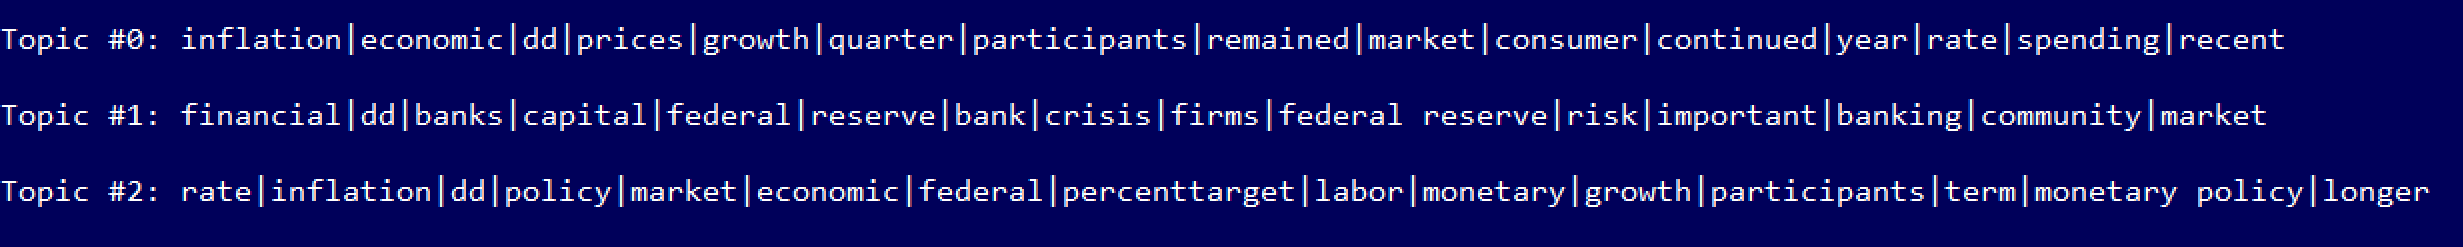
\includegraphics[width=\linewidth]{Topic-Model-3-topics.PNG}
  \caption{Top 15 Words Distributed Over Three Latent Topics}
  \label{fig:LDA}
\end{figure}

We found that the topic model generally distributed the speeches and minutes into the three categories fairly well.  It was interesting that "Topic 1" referred solely to financial stability, "Topic 0" primarily referred to inflation and spending, and "Topic 2" returned a word distribution that included labor, growth, and lower for longer monetary policy. \vertSpace

\subsubsection{Supervised Models}

We utilized the following models in our research: 

  \begin{itemize}

    \item Naive Bayes

      $$P(A|x_1,x_2,...,x_n) = p(A)\prod_{i=1}^n p(x_i|A)$$

    \item Logistic Regression

     $$A = \prod_{i=1}^n p(x_i)^{y_i}(1-p(x_i))^{1-y_i}$$

    \item Logistic Lasso
     $$A = \prod_{i=1}^n p(x_i)^{y_i}(1-p(x_i))^{1-y_i}+ L1$$
    \item SVM

     $$\left [\frac{1}{n} \sum_{i=1}^n max(0,1 - y_i(\vec{w} \dot \vec{x_i} - b)) \right] + \lambda ||\vec{w}||^2$$
    \item Neural Network
      We test a mixture of wide and deep neural nets. 
  \end{itemize}



\subsubsection{Basic Model Choice and Performance} 

The basic models are Naive Bayes, Logistic Regression, Logistic Lasso, and SVM.  We tested for model accuracy through averaging various iterations of each model's results, and we empirically tested for the optimal number of bigrams and anagrams.  \vertSpace


We found that the general accuracy of each model (for bigrams) peaked at around ten iterations of each model.  The F1 score, measured as the accuracy of predicting an FOMC move (up = down = 1) with bigrams, also peaks at around 10 iterations per model. \vertSpace


Given that the basic models are predicting binary classification we expected the Logistic Regression with L1 penalty (i.e., Logistic Lasso) to perform the best.  Based on empirical knowledge, FOMC rate moves are analyzed in terms of probabilities and the upcoming meeting is judged primarily on the outcome of Fed action or no action.  \vertSpace


Despite some good properties of SVM such as, SVM tend to perform better than logistic regression due to the face that SVMs are less sensitive to outliers and SVM try to maximize the margin between the closest support vectors while LR the posterior class probability. SVM generally find a solution which is as fare as possible for the two categories.  SVM provide prediction of 1 or 0, while the Logistic Regression provides a probability were a probability of 0.501 is enough for the prediction of FOMC rate action.  \vertSpace


In addition, because this is a binary classification problem, we also exptected Logistic Regression with L1 penalty (i.e., Logistic Lasso) to perform better than Logistic Regression without any regularization.  \vertSpace 

Given that we are modelling a classification problem, we would expect the performance of the Logistic Lasso model based on the mathematical properties of Logistic Lasso more robust for predicting FOMC rate action.  Logistic regression models the probability distribution of the class label $y$ given a feature vector $x$: 

$$p(y=1|x,\theta) = \sigma(\theta^T x) = \frac{1}{1+\exp(-\theta^Tx)}$$

The L1 regularized logistic regression (Logistic Lasso) is defined as: 

$$\underset{\rm \theta}{\rm min} \sum_{i=1}^M -\log p(y^{(i)}|x^{(i)}; \theta) + \beta ||\theta||$$

L1 regularization has the effect of forcing feature selection, and as we observe the Logistic Lasso model performs best Tri-grams to 7-grams and performance significantly drops with larger Ngrams.  \vertSpace 


Below is the average accuracy of the four basic classifiers (Naive Bayes, SVM, Logistic Regression, and Logistic Lasso) after 10 iterations: 

\begin{figure}[h!]
\begin{center}
\includegraphics[width=.3\textwidth]{"../output/data_for_graphs/log_lass_accuracy_more iterations".pdf}
\includegraphics[width=.3\textwidth]{"../output/data_for_graphs/log_reg_accuracy_more iterations".pdf}
\includegraphics[width=.3\textwidth]{"../output/data_for_graphs/NB_accuracy_more iterations".pdf}
\includegraphics[width=.3\textwidth]{"../output/data_for_graphs/SVM_accuracy_more iterations".pdf}
\end{center}
\end{figure}


\vspace{5cm}

\subsection{Feature Choice}

Based on previous research that applied Naive Bayes to analyzing FOMC transcripts \cite{stanford} ML models performed better with N-grams and performance peaked at tri-grams for Naive Bayes.  In our models, we found that N-grams of greater N saw greater accuracy and lower standard deviation.  


\begin{figure}[h!]
\begin{center}
\includegraphics[width=.3\textwidth]{"../output/data_for_graphs/log_lasso_f1".pdf}
\includegraphics[width=.3\textwidth]{"../output/data_for_graphs/log_f1".pdf}
\includegraphics[width=.3\textwidth]{"../output/data_for_graphs/naive_bayes_f1".pdf}
\includegraphics[width=.3\textwidth]{"../output/data_for_graphs/SVM_f1".pdf}
\end{center}
\end{figure}

As seen in the graphs above, the Logistic Lasso regression performs the best out of the four basic models.


 
% Bibliography
%-----------------------------------------------------------------
\begin{thebibliography}{99}

\bibitem{Cd94} Hansen,Stephen, McMachon, Michael  \emph{Transparency and Deliberation with the FOMC:a Computational Linquistics Approach}, CEPR Discussion Paper, (2014)

\bibitem{stanford} Puri, Indira \emph{Using Machine Learning to Predict Interest Rate Changes from Federal Reserve Proceedings}
\end{thebibliography}

\end{document}
